\documentclass[a4paper,twoside,11pt,titlepage]{report}

%------------------ PACKAGES ------------------------%

\usepackage{listings}
\usepackage[utf8]{inputenc}
\usepackage[spanish]{babel}
\usepackage[pdfborder={000}]{hyperref}
\usepackage{url}
\usepackage{longtable}
\usepackage{fancyhdr}
\usepackage{colortbl}
\usepackage{graphicx}
\usepackage{xspace}
\usepackage[nottoc]{tocbibind}
\usepackage[acronym,toc]{glossaries}
\usepackage{amsthm}
\usepackage{amsfonts}
\usepackage{acro}
\usepackage{hyperref}
\usepackage{graphicx}
\usepackage{float}
\usepackage{pgfplots}
\pgfplotsset{
  compat=1.12,
}

\decimalpoint
\usepackage{dcolumn}
\newcolumntype{.}{D{.}{\esperiod}{-1}}
\makeatletter
\addto\shorthandsspanish{\let\esperiod\es@period@code}
\makeatother

\usepackage{graphicx} %package to manage images
\graphicspath{ {imagenes/} }

\usepackage{appendix}
\renewcommand{\appendixname}{Anexos}
\renewcommand{\appendixtocname}{Anexos}
\renewcommand{\appendixpagename}{Anexos}

%------------------ REUSABLE INFORMATION ------------------------%

\newcommand{\myTitle}{Sistema de autenticación de doble factor basado en Criptografía de Curva Elíptica\xspace}
\newcommand{\myTitleEN}{Double authentication factor system based on Elliptic Curve Criptography\xspace}
\newcommand{\myDegree}{Grado en Ingeniería Informática\xspace}
\newcommand{\myName}{Sergio García Prados\xspace}
\newcommand{\myProf}{Antonio Francisco Díaz García\xspace}
\newcommand{\myFaculty}{Escuela Técnica Superior de Ingenierías Informática y de Telecomunicación\xspace}
\newcommand{\myFacultyShort}{E.T.S. de Ingenierías Informática y de Telecomunicación\xspace}
\newcommand{\myDepartment}{Departamento de Arquitectura y Tecnoloía de Computadores\xspace}
\newcommand{\myUni}{\protect{Universidad de Granada}\xspace}
\newcommand{\myLocation}{Granada\xspace}
\newcommand{\myTime}{\today\xspace}
\newcommand{\myVersion}{Version 0.1\xspace}
\newcommand{\myKeywords}{Criptografía, Sistemas operativos, C, Pluggable Authentication Module, Autenticación, Message Queuing Telemetry Transport, Seguridad, Criptografía de Curva Elíptica, Algoritmo de Firma Digital de Curva Elíptica\xspace}
\newcommand{\myKeywordsEN}{Criptography, Operative System, C, Pluggable Authentication Module, Authentication, Message Queuing Telemetry Transport, Security, Elliptic Curve Criptography, Elliptic Curve Digital Signature Algorithm\xspace}

%------------------ HEADERS AND FOOTERS ------------------------%

\pagestyle{fancy}
\fancyhf{}
\fancyhead[LO]{\leftmark}
\fancyhead[RE]{\rightmark}
\fancyhead[RO,LE]{\textbf{\thepage}}
\renewcommand{\chaptermark}[1]{\markboth{\textbf{#1}}{}}
\renewcommand{\sectionmark}[1]{\markright{\textbf{\thesection. #1}}}

%------------------ PAGE STYLE ------------------------%

\setlength{\headheight}{1.5\headheight}
\newcommand{\HRule}{\rule{\linewidth}{0.5mm}}

%------------------ EXMAPLES AND DEFINITIONS ------------------------%
\newtheorem{ejemplo}{Ejemplo}[chapter]
\newtheorem{definicion}{Definición}[chapter]

%------------------ COLORS ------------------------%
\definecolor{gray97}{gray}{.97}
\definecolor{gray45}{gray}{.45}
\definecolor{gray30}{gray}{.94}

%------------------ NON-FORMATTED TEXT ------------------------%

\lstset{ frame=Ltb,
    framerule=0.5pt,
    aboveskip=0.5cm,
    framextopmargin=3pt,
    framexbottommargin=3pt,
    framexleftmargin=0.1cm,
    framesep=0pt,
    rulesep=.4pt,
    backgroundcolor=\color{gray97},
    rulesepcolor=\color{black},
    %
    stringstyle=\ttfamily,
    showstringspaces = false,
    basicstyle=\scriptsize\ttfamily,
    commentstyle=\color{gray45},
    keywordstyle=\bfseries,
    %
    numbers=left,
    numbersep=6pt,
    numberstyle=\tiny,
    numberfirstline = false,
    breaklines=true,
}

% minimizar fragmentado de listados
\lstnewenvironment{listing}[1][]
{\lstset{#1}\pagebreak[0]}{\pagebreak[0]}

\lstdefinestyle{CodigoC}
{
  basicstyle=\scriptsize,
  frame=single,
  language=C,
  numbers=left
}

\lstdefinestyle{Consola}
{
  basicstyle=\scriptsize\bf\ttfamily,
  backgroundcolor=\color{gray30},
  frame=single,
  numbers=none
}

%------------------ REDEFINE MACRO ------------------------%
%Para conseguir que en las páginas en blanco no ponga cabeceras
\makeatletter
\def\clearpage{%
  \ifvmode
    \ifnum \@dbltopnum =\m@ne
      \ifdim \pagetotal <\topskip
        \hbox{}
      \fi
    \fi
  \fi
  \newpage
  \thispagestyle{empty}
  \write\m@ne{}
  \vbox{}
  \penalty -\@Mi
}
\makeatother

\theoremstyle{definition}
\newtheorem{definition}{Definition}[section]

%------------------ ACRONIMOS ------------------------%

\makeglossaries
\newacronym{rae}{RAE}{Real Academia Española}
\newacronym{cpd}{CPD}{Centros de Procesamiento de Datos}
\newacronym{pam}{PAM}{Pluggabe Authentication Module}
\newacronym{mqtt}{MQTT}{Message Queueing Transport Telemetry}
\newacronym{ssh}{SSH}{Secure Shell}
\newacronym{sha}{SHA}{Secure Hash Algorithm}
\newacronym{ecdsa}{ECDSA}{Elliptic Curve Digital Signature Algorithm}
\newacronym{tls}{TLS}{Transport Layer Security}
\newacronym{iot}{IoT}{Internet of Things}
\newacronym{puf}{PUF}{Physical Unclonable Functions}
\newacronym{ttp}{TTP}{Trusted Third Party}
\newacronym{jwt}{JWT}{JSON Web Token}
\newacronym{ecc}{ECC}{Elliptic Curve Criptography}
\newacronym{otp}{OTP}{One Time Password}
\newacronym{hmac}{HMAC}{Hash Message Authentication Code}
\newacronym{totp}{TOTP}{Time-based One Time Password}
\newacronym{sso}{SSO}{Single Sign-On}
\newacronym{mfa}{MFA}{Multiple Factor Authentication}
\newacronym{pki}{PKI}{Public Key Infrastructure}
\newacronym{http}{HTTP}{Hyper Text Transfer Protocol}
\newacronym{rsa}{RSA}{ivest-Shamir-Adleman}
\newacronym{ansi}{ANSI}{American National Standards Institute}
\newacronym{dlp}{DLP}{Discrete Logarithm Problem}
\newacronym{ecdlp}{ECDLP}{Elliptic Curve Discrete Logarithm Problem}
\newacronym{ftp}{FTP}{File Transport Protocol}
\newacronym{rlogin}{Rlogin}{Remote Login}
\newacronym{api}{API}{Application Program Interface}
\newacronym{spi}{SPI}{Service Provider Interface}
\newacronym{ca}{CA}{Cerificate Authority}
\newacronym{csr}{CSR}{Certificate Signing Request}
\newacronym{uuid}{UUID}{Universally Unique IDentifier}
\newacronym{scp}{SCP}{Secure Copy Protocol}
\newacronym{mitm}{MITM}{Man In The Middle}
\glsaddall

%------------------ DOCUMENT ------------------------%
\begin{document}

\renewcommand{\listtablename}{Índice de tablas}
\renewcommand{\tablename}{Tabla}

\begin{titlepage}
    \newlength{\centeroffset}
    \setlength{\centeroffset}{-0.5\oddsidemargin}
    \addtolength{\centeroffset}{0.5\evensidemargin}
    \thispagestyle{empty}

    \noindent\hspace*{\centeroffset}\begin{minipage}{\textwidth}

        \centering
        
\includegraphics[width=0.9\textwidth]{imagenes/logo_ugr.jpg}\\[1.4cm]

        %------------------ UPPER PART ------------------------%
        \textsc{\Large TRABAJO FIN DE GRADO\\[0.2cm]}
        \textsc{\myDegree\\[1cm]}

        %------------------ TITLE ------------------------%
        {\Huge\bfseries Sistema de autenticación de doble factor basado en Criptografía de Curva Elíptica\\}
    \end{minipage}

    \vspace{1.5cm}

    \noindent\hspace*{\centeroffset}\begin{minipage}{\textwidth}
        \centering

        \textbf{Autor}\\ {\myName}\\[2.5ex]
        \textbf{Director}\\ {\myProf}\\[2cm]
        
\includegraphics[width=0.3\textwidth]{imagenes/etsiit_logo.png}\\[0.1cm]
        \textsc{\myFaculty}\\
        \textsc{---}\\
        Granada, \myTime
    \end{minipage}
\end{titlepage}
%------------------ KEY WORDS - ABSTRACT (ESP) ------------------------%

\thispagestyle{empty}

\cleardoublepage

\begin{center}
    {\large\bfseries \myTitle}\\
\end{center}

\begin{center}
    \myName\\
\end{center}

\noindent{\textbf{Palabras clave}: \myKeywords}\\

\vspace{0.7cm}

\noindent{\textbf{Resumen}}\\

Cada vez está más en boca el término ``seguridad''. No es de extrañar que desde que comenzó la era digital, los retos tecnológicos 
son cada vez más complejos. No obstante, dado el grado de conocimiento y herramienta de las que disponemos, estos son bastante 
factibles y llamativos para cualquiera. Es por eso que el uso de elementos tecnológicos en nuestro día a día se
concibe como algo innato en nuestras vidas. 

La tecnología nos trae numerosos beneficios. Nada más que con echar la vista atrás y ver como la sociedad ha llegado a conseguir 
retos tan importantes gracias a la ayuda de esta es suficiente. Sin embargo, la tecnología tiene su lado adverso, la seguridad. 
Por muy llamativa y útil que pueda ser una tecnología, si no se lleva a cabo unos cumplimientos de seguridad bien definidos
y estrictos durante su desarrollo, el usuario final puede no llegar a usarlo y por tanto quedar en vano el trabajo realizado o 
peor aun, que sea usado muchos usuarios y tengas graves vulnerabilidades que afecten a la integridad de sus datos.

Con la llegada del \textit{Big Data}, cada vez más tenemos acceso a cualquier información en cualquier momento. Las compañías 
hacen un arduo esfuerzo en proteger nuestros datos y que estos no caigan en las manos equivocadas. Pero como bien es de saber, 
ningún sistema, por muy complejo y sofisticado que pueda llegar a ser, es 100\% seguro. Cada día salen nuevas vulnerabilidades
y complejos ataques para corromper estos sistemas y es por ello que la inversión de las compañías en ciberseguridad incrementa
cada año. Para que esta inversión sea eficiente, es necesario apostar por la investigación en este campo y así garantizar un 
futuro más ``seguro''.

El objetivo de este trabajo es el estudio de la seguridad en entornos definidos (\acf[first-style=short]{hpc} y Cloud) donde el volumen de datos 
que se almacena es elevado y por consiguiente puede ser información más sensible, garantizando la confidencialidad, integridad y 
disponibilidad del sistema.  

Se propone una solución \cite{multipauthpaper} de un modelo de autenticación multifactor, \acf[first-style=short]{mfa}, basada en un sistema 
electrónico (MCU basado en un ESP-32) garantizando un alto rendimiento y eficiencia debido al consumo de estos componentes electrónicos,
una arquitectura distribuida ofreciendo una mayor escalabilidad y con un alta granularidad en cuanto a seguridad se refiere. 

Este trabajo se centra principalmente en la incorporación de un modulo de seguridad a este sistema de autenticación propuesto de 
forma que pueda ser usado por cualquier otro dispositivo en entornos variados garantizando una solución portable y eficiente.

%------------------ KEY WORDS - ABSTRACT (EN) ------------------------%

\thispagestyle{empty}

\cleardoublepage

\begin{center}
    {\large\bfseries \myTitleEN}\\
\end{center}

\begin{center}
    \myName\\
\end{center}

\noindent{\textbf{Keywords}: \myKeywordsEN}\\

\vspace{0.7cm}

\noindent{\textbf{Abstract}}\\


The term ``security'' is becoming more and more popular. It is not surprising that since the digital era began, technological 
challenges have become increasingly complex. However, given the degree of knowledge and tools at our disposal, they are quite 
feasible and appealing to anyone. That is why the use of technological elements in our daily lives is conceived as something 
innate in our lives. 

Technology brings us numerous benefits. Just looking back and seeing how society has achieved such important challenges thanks to 
its help is enough. However, technology has its downside: security. No matter how attractive and useful a technology may be, if it 
does not comply with well-defined and strict security standards during its development, the end user may not use it and therefore 
the work done may be in vain, or worse still, it may be used by many users and have serious vulnerabilities that affect the 
integrity of their data.

With the advent of \textit{Big Data}, we increasingly have access to any information at any time. Companies make an arduous effort 
to protect our data from falling into the wrong hands. But as we all know, no system, no matter how complex and sophisticated it 
may be, is 100\% secure. Every day new vulnerabilities and complex attacks to corrupt these systems emerge and that is why 
companies' investment in cybersecurity increases every year. In order for this investment to be efficient, it is necessary to 
invest in research in this field and thus guarantee a more ``secure'' future.

The objective of this work is the study of security in defined environments (\acf[first-style=short]{hpc} and Cloud) where the volume of data 
stored is high and therefore may be more sensitive information, ensuring the confidentiality, integrity and availability of the 
system.  

A solution \cite{multipauthpaper} of a multifactor authentication \acf[first-style=short]{mfa} model is provided, based on an electronic system 
(MCU based on ESP-32) guaranteeing high performance and efficiency due to the consumption of these electronic components, a distributed 
architecture offering greater scalability and with a high granularity in terms of security. 

This work is mainly focused on the incorporation of a security module to this proposed authentication system so that it can be 
used by any other device in varied environments guaranteeing a portable and efficient solution.

%------------------ AUTORIZACION ------------------------% 

\thispagestyle{empty}

\cleardoublepage

\noindent\rule[-1ex]{\textwidth}{2pt}\\[4.5ex]

Yo, \textbf{\myName}, alumno de la titulación \myDegree de la \textbf{\myFaculty de la \myUni}, con DNI 77148519X, autorizo la
ubicación de la siguiente copia de mi Trabajo Fin de Grado en la biblioteca del centro para que pueda ser
consultada por las personas que lo deseen.

\vspace{6cm}

\noindent Fdo: \myName

\vspace{2cm}

\begin{flushright}
Granada a \myTime
\end{flushright}

\chapter*{}

\thispagestyle{empty}

\noindent\rule[-1ex]{\textwidth}{2pt}\\[4.5ex]

D. \textbf{\myProf}, Profesor del \myDepartment de la \myUni.

\vspace{0.5cm}

\textbf{Informan:}

\vspace{0.5cm}

Que el presente trabajo, titulado \textit{\textbf{\myTitle}}, ha sido realizado bajo su supervisión por \textbf{\myName}, y autorizamos la defensa de dicho trabajo ante el tribunal
que corresponda.

\vspace{0.5cm}

Y para que conste, expiden y firman el presente informe en Granada a \myTime.

\vspace{1cm}

\textbf{El director:}

\vspace{5cm}

\noindent \textbf{\myProf}

%------------------ AGRADECIMIENTOS ------------------------% 

\thispagestyle{empty}

\cleardoublepage

\chapter*{Agradecimientos}

\vspace{1cm}

A mi director de Trabajo Fin de Grado, \myProf  por su coordinación y conocimiento acerca de la materia que me ha ayudado a 
desarrollar este trabajo a pesar de los inconvenientes.

Tambien me gustaría agradecer este trabajo al apoyo de mi madre y hermanos que han confiado en mi en todo momento y me han dado 
soporte en los momentos mas dificiles de mi recorrido académico. Pero sobre todo a mi padre, que ha sido mi apoyo incondicional en 
estos años de carrera y del que seguro que estaría orgulloso de ver lo lejos que he llegado.

¡Gracias!


\tableofcontents
\listoffigures
\listoftables

\chapter{Introducción}

El concepto de ``Seguridad de la Información'' se acuñó por primera vez en un artículo del Instituo Nacional de Estándares y 
Teconología (\acf[first-style=short]{nist}) en 1997 \cite{neumann1977post} aunque la seguridad en el campo de la tecnología siempre ha estado en 
boca de todos y ha sido un apsecto a tener en cuenta. 

La ciberseguridad se empezó a tener en cuenta con el ``\textit{boom}'' de la era digital. No obstante, habría que remontarse unos 
siglos atras para saber cuando se empezó a aplicar métodos seguros a la información. Concretamente cuando Julio César vivía, se 
empezó a usar algoritmos de cifrado simples que se aplicaban sobre mensajes que tenían que ser enviados y así si alguien lo 
interceptada, no podía saber su contenido. A esta práctica se conoce como criptografía. La criptografía ha estado latente en muchos 
hitos de nuestra historia, como por ejemplo con la aparición Alang Turing y su ingenio para descifrar las comunicaciones entre 
integrantes del ejército alemán en código morse.

La criptografía, según la \acf[first-style=short]{rae} es el ``arte de escribir con clave secreta o de un modo enigmático''. Esta herramienta
ha sido la base de la seguriadad de la información ya que sustenta las tres propiedades de todo sistema seguro (CIA): confidencialidad 
(\textit{confidenciality}), integridad (\textit{integrity}) y disponibilidad (\textit{availability}).

Tal y como se puede apreciar en \cite{digital_attack}, el número de ciberataques que suceden a diaría es muy elevado. Es por ello
que se cualquier empresa que de soporte a clientes almacenando información sensible use herramientas de seguridad que estén al 
día de los distintas vulnerabilidades que se descubren \cite{cve_mitre}.

\section{Motivación}
\label{sec:motivacion}

La idea de este tarbajo nace de a raiz de la tesis doctoral \cite{tesisIliaBlockin} publicada en 2020 por la Universidad de Granada
titulada ``\textit{Mecanismos de seguridad para Big Data basados en circuitos criptográficos}'' y elaborada por \textit{Ilia 
Blockin}. Esta tesis sugiere soluciones basada en sistemas electrónicos que ofrecen una solución eficiente y flexible para 
aumentar la seguridad en el acceso a servicios y sistemas que pueden procesar gran cantidad de información. 

El planteamiento se detalla en unos de las mejoras propuestas de dicha tesis: ``\textit{continuar mejorando los sistemas propuestos 
agregando compatibilidad con otros métodos de autenticación como el Módulo de autenticación conectable de Linux (PAM) u otros 
protocolos de autenticación}'' 

Personalmente, me he decantado por la elección de este tema ya que tengo especial interés en el campo de la ciberseguridad y por 
el reto de conocer en profundidad las bases de la criptografía.

\section{Objetivos}

Para elaborar la lista de objetivos, es necesario conocer los requisitos del sistema donde se pretende implantar. Este entorno
viene descrito de forma detallada en \cite{multipauthpaper}. 

\subsection{Diseño del sistema propuesto}

Se propone un sistema con un conjunto de elementos físicos y virtualizados:

\begin{itemize}
    \item \textit{Usurio}: quien accede al sistema
    \item \textit{Servicios}: ofrecido por programas a través de conexión TCP 
    \item \textit{Servidores}: ordenadores donde los servicios son instalados
    \item \textit{Clientes}: ordenadores desde donde los servicios son accedidos
    \item \textit{eToken}: dispositivos que autentica la petición del usuario
\end{itemize}

Se define una lista de control (\acf[first-style=short]{acl}) con reglas para garantizar una autorización deseada. Cada elemento viene 
identificado por un Identificador Único Universal (\acf[first-style=short]{uuid}) de 128 bits y un par de claves pública y privada que permite 
al sistema a autenticar las peticiones.
El sistema es híbrido, es decir que usan la clave pública combinado con un modelo centralizado para autorizar el acceso. Hay 
dos elementos más:

\begin{itemize}
    \item \textit{Servidor de configuración}: permite modificar la configuración de cada elemento remotamente
    \item \textit{Servidor de autenticación}: autoriza la petición de acceso a servicios basado en las ACL
    \item \textit{Gateway}: redirige la conexión de red entre clinte y servidores
    \item \textit{Broker MQTT}: servidor de intercambio de mensajes 
\end{itemize}

\subsection{Listado de objetivos}

El presente trabajo conlleva el cumplimiento de los siguientes objetivos:

\begin{enumerate}
    \item Crear un módulo \acf[first-style=short]{pam} para el sistema de autenticación propuesto en \cite{multipauthpaper}
    \item Implementar el módulo PAM para el servicio \acf[first-style=short]{ssh}
    \item Usar el protocolo \acf[first-style=short]{mqtt}
    \item Seguir esquema de autenticación \textit{challenge-response} \cite{newman2010salted}
    \item Cifrar el \textit{challenge} mediante un algoritmo de cifrado unidireccional robusto como por ejemplo SHA512 
    (\acf[first-style=short]{sha})
    \item Usar Criptografía de Curva Elíptica o \acf[first-style=short]{ecc} tanto para la firma del \textit{challenge} como para la verificación 
    del mismo usando el Algoritmo de Firma Digital de Curva Elíptica (\acf[first-style=short]{ecdsa})
    \item Encriptar las comunicaciones entre los elementos del sistema propuesto usando \acf[first-style=short]{tls} versión 1.2
\end{enumerate}

\section{Estructura del trabajo}

El presente trabajo se divide en las siguientes capítulos: en el Capítulo \ref{chap:estado-arte} se detalla la ``situación actual de la 
tecnología''. Se habla de otros proyectos que existen actualmente y que realizan funcionalidades iguales o parecidas a las 
que se propone en este proyecto. Se valora los puntos fuertes y ámbitos en los que se puede aplicar. En el Capítulo \ref{chap:analisis-problema},
se habla de la seguridad en el apartado de la autenticación en sistemas, la seguridad aplicada a entornos IoT, el protocolo
MQTT usado, la criptografía de curva elíptica y el algoritmo ECDSA y por último PAM y su arquitectura. Al final se hace alusión
de las herramientas usadas para el desarrollo de este trabajo. En el Capítulo \ref{chap:diseño} se hace un análisis exhaustivo del 
funcionamiento del programa indicando sus distintas fases. En el Capítulo \ref{chap:analisis-seguridad} lista algunas caracterísiticas
de seguridad y cómo las lleva a cabo. En el Capítulo \ref{chap:presupuesto} se hace un resumen de lo que ha costado económicamente el 
proyecto y su desarrollo temporal con un diagrama de Gantt. Por último, en el Capítulo \ref{chap:conclusion} se hace un resumen de objetivo
de este proyecto, los resultado obtenidos, problemas afrontados y futuras mejoras.
\chapter{Estado del arte}
\label{chap:estado-arte}

Vamos a enfocar los trabajos relacionados con respecto a la seguridad que ofrece la Criptografía de Curva Elíptica en dispositivos
electrónicos para proporcionar un método de autenticación de doble factor. Los trabajos citados a continuación son comparados
con el propuesto en \cite{multipauthpaper}. \textit{Braeken} propone en \cite{braeken2018puf} un protocolo de autenticación para 
dispositivos \acf[first-style=short]{iot} basado en una función física no clonable \acf[first-style=short]{puf}. Ambos sistemas se caracterizan porque usan
un esquema de acuerdo de claves en el que cualquier nodo está registrado bajo la supervisión de un tercer elemento de 
confianza \acf[first-style=short]{ttp} y el uso de certificados. Además, en ambos sistemas se usa el mecanismo de autenticación basado en 
reto-respuesta (\textit{challenge-response}). En este, una entidad se autentica enviando un valor dependiente
de un valor secreto y un valor desafío cambiante \cite{van2014encyclopedia}. Si la respuesta es correcta, se da por légitimo al 
cliente y se autentica. El sistema prouesto en \cite{multipauthpaper} a diferencia de \cite{braeken2018puf}, usa el protocolo 
\acf[first-style=short]{mqtt} para la comunicación entre los dispositivos de tal forma que lo hace más escalable. 

\textit{Gao} \cite{gao2020scitokens} propone un sistema similar que usa un token de autenticación basado en el formato JSON, 
\acf[first-style=short]{jwt}, junto al servicio SSH y desarrolla, al igual que lo que se propone en el presente trabajo, un módulo PAM de tipo
desafio-respuesta. Sin embargo, a diferencia de \cite{gao2020scitokens}, este trabajo no usa un formato concreto para responder
al desafio. De manera similar a \cite{braeken2018puf}, tmapoco implementa el protocolo MQTT para la comunicación  entre los 
nodos que intervienen. 

Existen otros sistemas como por ejemplo el propuesto por \textit{Fayad} en \cite{fayad2020secure} que ratifica la robustez que 
tiene ECC sobre otros mecanismos de autenticacion como las contraseñas de un solo uso (\acf[first-style=short]{otp}) basadas en mensajes 
\textit{Hash} (\acf[first-style=short]{hmac}) o basadas en tiempo (\acf[first-style=short]{totp}) para entornos con dispositivos IoT. 

Actualmente, existen múltiples métodos de autenticación bien definidos que cumplen con los parametros requeridos: algo que sabes
(contraseña), algo que tienes (token) y algo que eres (biometría). Para que sea multifactor, al menos dos parametros tienen que
ser requeridos. Google creó un módulo PAM \cite{noauthor_googlegoogle-authenticator-libpam_2021} para garantizar un factor de 
serguridad en la autenticación usando su producto \textit{Google Authenticator}. Por otra parte, existen productos como llaves físicas
de autenticación que verifican tu identidad usando protocolos de seguridad robustos. Es el caso por ejemplo de Yubikey 
\cite{noauthor_yubikey_nodate}. A diferencia del sistema propuesto, la verificación por llave de seguridad requiere del dispositivo
físico. También hay productos software en el mercado que permiten el acceso seguro a sistemas sin la necesidad de tener que 
proveer de la metodología clásica par usario-contraseña. El inicio de sesión único o \acf[first-style=short]{sso} \cite{noauthor_single_nodate}
es un método de autenticación que permite a los usuarios autenticarse de forma segura en múltiples aplicaciones y servicios web 
usando un único conjunto de credenciales.

\chapter{Análsis del problema}
\label{chap:analisis-problema}

\section{Seguridad en la autenticación}

La autenticación del usuario es el punto de entrada a diferentes redes o instalaciones informáticas en las que se presta un 
conjunto de servicios a los usuarios o se puede realizar un conjunto de tareas. 

Una vez autenticado, el usuario puede acceder, por ejemplo a la Intranet de una empresa, a consolas, bases de datos, edificios 
vehículos, etc. La usabilidad de los mecanismos de autenticación se investiga cada vez con más detenimiento y dado que los 
estos son concebidos, implementados, puestos en práctica y corrompidos por teceras personas, hay que tener en cuenta los factores 
humanos en su diseño. 

Actualmente existen múltiples métodos para autenticar a un usuario contra un sistema, siendo el más común es el par de claves 
usuario y contraseña, pero no es el único. El uso de certificados está cada vez más extendido en Infraestructuras de Clave 
Pública (\acf[first-style=short]{pki}). 

Para garantizar que un sistema es necesario que se garantizen tres aspectos \cite{bases_seguridad}:

\begin{itemize}
    \item \textit{Confidencialidad}: prevenir la divulgación no autorizada de la información
    \item \textit{Integridad}: prevenir modificaciones no autorizadas de la información
    \item \textit{Disponibilidad}: prevenir interrupciones no autorizadas de los recursos informáticos
\end{itemize}

Usar un método de autenticación no implica que el sistema sea completamente seguro. De echo, la autenticación se convierte en 
un proceso más robusto y fiable aplicando múltiples métodos, también llamado \acf[first-style=short]{mfa}. Este mecanismo propone tres tipos 
de factores que permiten a un usuario vincularlo con las credenciales establecidas \cite{ometov2018multi}:

\begin{enumerate}
    \item \textit{Factor conocimiento}: algo que el usuario conoce (contraseña)
    \item \textit{Factor pertenencia}: algo que el usuario tiene (token)
    \item \textit{Factor biometrico}: algo que el usuario es (huella dactilar) 
\end{enumerate}

La autenticación basada en múltiples factores provee un nivel de seguridad elevado y facilita una protección continua de 
dispositivos y otros servicios críticos ante accesos no autorizados usando dos o más factores.

Además de la robustez de la seguridad durante el proceso de autenticación, la usabilidad se convierte a su vez en una cuestión 
estratégica en el establecimiento de métodos de autenticación de  usuarios.

La usabilidad puede definirse como ``la medida en que un producto puede ser utilizado por determinados usuarios para alcanzar 
determinados objetivos con eficacia, eficiencia y satisfacción en un contexto de uso específico''. La usabilidad de la seguridad se 
ocupa del estudio de cómo debe tratarse la información de seguridad en la interfaz de usuario y de cómo deben ser los mecanismos 
de seguridad y los sistemas de autenticación deben ser fáciles de usar \cite{braz2006security}.

Este sistema \cite{multipauthpaper} propone un mecanismo de autenticación usable, de múltiples factores y escalable gracias 
principalmente al uso de dispositivos electrónicos con circuitos integrados como es Arduino así como del protocolo MQTT.

\subsection{Seguridad en IoT}

El Internet de las cosas (\acf[first-style=short]{iot}) es un término relativamente nuevo. Se puede definir como una red abierta y completa de 
objetos inteligentes que tienen la capacidad de auto-organizarse, compartir información, datos y recursos, reaccionar y actuar 
ante situaciones y cambios en el entorno \cite{madakam2015internet}. 

El IoT ha facilitado la interconectividad entre dispositivos ayudando a conectar sensores, vehículos, hospitles, industrias y 
consumidores a través de Internet. Las arquitecturas en IoT son cada vez más complejas, descentralizadas y fluidas dado el 
incremento de dispositivos que se comunuican entre sí y es por ello que la seguridad juega un papel fundamental en él. 
Los dispositivos IoT deben ser seguros y no pueden ser manipulados por terceras personas no autorizadas. 

\subsection{\acf[first-style=short]{mqtt}}

Es un protocolo de comunicación que funciona a nivel de la capa de aplicación. Es usado principalmente en entornos
con dispositivos IoT por ser un protocolo con un consumo de bando de ancha y batería mínimo \cite{sugumar2020mqtt}.

A diferencia del protoclo de comunicación \acf[first-style=short]{http} que funciona mediante petición-respuesta, MQTT está basado es 
publicación-respuesta. Este modelo de protocolo requiere de un broker mensajero. Existen múltiples tipos de brokers como 
Mosquitto \cite{eclipse_2018}, HiveMqtt \cite{hivemq}, Mosca \cite{moscajsmosca_2021}, cloudMQTT \cite{cloudmqtt}, MQTT.Js 
\cite{mqttjs}, etc. Para el trabajo propuesto, se usa Mosquitto.

\subsubsection{Funcionamiento del protocolo MQTT}

El cliente MQTT se conecta el broker MQTT subscribiéndose a un tópico. Un tópico es un identificador al cual los nodos se subscriben
y por el que publican mensajes. Si algun mensaje es publicado por un tópico, este llega a todos los nodos que estés suscritos al 
mismo. Se representa con una cadena de caracteres separada por el símbolo $/$ indicando el elemento, dentro de una jerarquía, al 
que se subscribe. 
Un ejemplo de un tópico sería $cocina/sensor1/temperatura$ de tal forma que el cliente obtiene la información de temperatura que 
le llega el sensor1 en la cocina. MQTT se basa en el protoclo TCP/IP para la transmisión de datos. 
El cliente siempre interactua con el broker. No obstante, puede haber múltiples brokers que intercambien datos segun los 
tópicos de subscripción.

\subsubsection{Seguridad en MQTT}
Para garantizar un nivel de seguridad elevado en cuanto a la transmisión de datos se refiere, este protocolo usa por encima
TLS para garantizarlo. Este protolo crea un canal seguro entre el cliente y el broker, parecido a como funciona en los 
navegadores web. Para ello es necesario un certificado del servidor de confianza. 

\subsubsection{Ventajas de MQTT sobre HTTP}

En HTTPS, no se mantiene una conexión continua. El cliente tiene que mandar petición de sondeo (\textit{poll request}) donde 
este solicita información al servidor acerca de la nueva petición de conexión TCP así como la negociación del tipo de 
encriptación SSL/TLS. 

A diferencia de HTTPS, MQTT establece una única conexión inicial. MQTT mantiene un flujo de mensajes fijo (\textit{keep alive})
entre aplicaciones sobre la conexión TCP de tal forma que las aplicaciones pueden detectar cuando una conexión está rota.

\subsection{Criptografía de Curva Elíptica}

La Criptografía de Curva Elíptica (\acf[first-style=short]{ecc}) pertenece a las tres familias de algoritmos de clave pública de gran relevancia 
(factorización de enteros, logaritmos discretos y curva elíptica). Este último nació entorno a mitad de los años 80.
ECC provee del mismo nivel de seguridad que \acf[first-style=short]{rsa} o sistemas logarítmicos discretos con operaciones considerablemente 
pequeñas. ECC está basado en el problema de logaritmo discreto (\acf[first-style=short]{dlp}) \cite{mccurley1990discrete}. ECC tiene beneficios 
en cuanto a su capacidad computacional ya que requiere de menos operaciones computacionales y tiene un consumo de ancho de banda 
muy inferior debido a la pequeña longitud de las claves y firmas con respecto otros como RSA. Esto lo hace ídoneo en arquitecturas
que intervienen dispositivos electrónicos de bajo consumo (Arduinos, Raspberry Pi, etc). No obstante, las operaciones RSA que 
implican una clave pública más pequeña son más rápidas que ECC.

El objetivo de esta sección es explicar las bases de este algoritmo sin entrar en detalles matemáticos. Para mayor documentación
se sugiere leer el libro \cite{paar2009understanding} del cual se ha sacado la información.

Esta sección se distribuye de la siguiente manera: definición del concepto de curva elíptica, problema de logaritmo discreto 
aplicado a las curvas elípticas, algoritmo ECDSA y comparativa con RSA.

\subsubsection{Definición de curva elíptica}

De las ecuaciones polinómicas de una circunferencia y una elipse se pueden sacar diferentes tipos de curvas. Las curva elíptica
es un tipo especial de ecuación polinómica. En criptografía se trabaja sobre un conjunto de números finitos, más popularmente
campos primo, donde todas las operaciones aritméticas se desarrollan sobre módulo \textit{p}, siendo este un número primo.

La definición de curva elíptica es la siguiente:

\begin{definition}[Curva Elíptica]
    La curva elíptica sobre $\mathbb{Z}_{p}$, $\textit{p} > 3$, es el conjunto de pares de punto $\textit{(x,y)} \in \mathbb{Z}_{p}$ 
    que cumplen 
    \begin{equation}
        y^2 = x^3 + ax + b \; mod \; p
    \end{equation}
    junto a un punto infinito imaginario \textit{O}, donde 
    \begin{equation}
        a, b \in \mathbb{Z}_{p}
    \end{equation} 
    y la condición
    \begin{equation}
        4a^3 + 27b^2 \not = 0 \; mod \; p
    \end{equation}
\end{definition}

Ejemplo de una curva elíptica:

\begin{figure}[H]
    \centering
    \begin{tikzpicture}
        \begin{axis}[
                xmin=-2,
                xmax=4,
                ymin=-7,
                ymax=7,
                xlabel={$x$},
                ylabel={$y$},
                scale only axis,
                axis lines=middle,
                % set the minimum value to the minimum x value
                % which in this case is $-\sqrt[3]{7}$
                domain=-1.912931:3,      % <-- works for pdfLaTeX and LuaLaTeX
                samples=200,
                smooth,
                % to avoid that the "plot node" is clipped (partially)
                clip=false,
                % use same unit vectors on the axis
                axis equal image=true,
            ]
            \addplot [red] {sqrt(x^3+7)}
            node[right] {$y^2=x^3+7$};
            \addplot [red] {-sqrt(x^3+7)};
        \end{axis}
    \end{tikzpicture}
    \caption{Representación gráfica de una curva elíptica}
\end{figure}

Aspecto fundamentales a tener en cuenta de la curva:

\begin{itemize}
    \item Es una curva no-singular, es decir que la curva no se intersecta a si mismo siempre y cuando el discriminante de la curva
    $-16(4a^3 + 27b^2) \not = 0$
    \item La curva es simétrica con respecto al eje de abscisas ya que si despejamos la $y$ de la ecuación obtenemos dos soluciones
    $\pm\sqrt{x^3 + ax + b} \; mod \; p$ 
    \item Hay solo una intersección en el eje de abscisas. Se debe a que si solucionamos la ecuación para $y = 0$, exite una 
    solución real (intersección con el eje de abscisas) y dos soluciones complejas (no mostradas en la gráfica). Existen curvas 
    elípticas con tres soluciones reales.
\end{itemize}

\subsubsection{\acf[first-style=short]{ecdsa}}
\label{subsec:ecdsa}

La curva elíptica tiene ventajas sobre RSA y otros esquemas DL. Los ECC con una clave con un tamaño que oscila entre los 160 y 256
bits proveen de una seguridad similar a otros algoritmos criptográficos de entre 1024 y 3072 bits. Esta propiedad resulta en un 
tiempo de procesamiento menor así como firmas más pequeñas. Por esa razón, ECDSA fue estandarizado en Estados Unidos por la 
\acf[first-style=short]{ansi} en 1998. 
El estándar ECDSA es definido para curvas elípticas sobre campos de número primo $\mathbb{Z}_{p}$ y campos de Galois $GF(2^m)$.
Este algorimo se compone de las siguientes fases:

\begin{enumerate}
    \item Generación de claves. Estas deben ser de al menos 160 para un nivel de seguridad elevado
    \item Generación de firma. Usa la clave privada para generar una pareja de valores enteros $(r,s)$. Usa 
    \item Verificación de firma. Usa la clave pública junto al par $(r,s)$ y un valor concreto.
\end{enumerate}

\subsubsection{Seguridad sobre ECDSA}
Suponiendo que los parámetros de la curva elíptica son escogidos correctamente, el principal ataque analíico sobre ECDSA intentaría
resolver el problema de logaritmo discreto de curva elíptica. Si un atacante fuera capaz de llevarlo acabo, podría resolver la 
clave privada y/o la clave efímera. No obstante, el mejor ataque conocido contra ECDSA tiene una complejidad proporcional a la 
raiz cuadrada del tamaño del grupo sobre el cual el DL es definido. El parámtero de ECDSA y su correspondiente nivel de seguridad 
están definidos en la tabla \ref{tab:bit-len-sec-level}

\begin{table}[H]
    \centering
    \begin{tabular}{ |c|c|c| }
        \hline
        \textit{Tamaño número primo q} & \textit{Tamaño hash} & \textit{Nivel de seguridad} \\
        \hline
        192                            & 192                  & 96                          \\
        224                            & 224                  & 112                         \\
        256                            & 256                  & 128                         \\
        384                            & 384                  & 192                         \\
        512                            & 512                  & 256                         \\
        \hline
    \end{tabular}
    \caption{Tamaño de bits y nivel de seguridad de ECDSA}
    \label{tab:bit-len-sec-level}
\end{table}

El algoritmo ECDSA requiere de claves mas pequeñas para proporcionar la misma robustez que otras como por ejemplo RSA. En la
tabla \ref{tab:rsa-vs-ecdsa} se detalla la comparación entre claves de ambos algoritmos de encriptación:

\begin{table}[H]
    \centering
    \begin{tabular}{ |c|c|c| }
        \hline
        \textit{Tamaño clave RSA} & \textit{Tamaño clave ECDSA} & \textit{Curva ESP\_IDF}        \\
        \hline
        1024 bits                 & 160-223 bits                & secp192r1, sec192k1           \\
        2048 bits                 & 224-255 bits                & secp224r1, sec224k1           \\
        3072 bits                 & 256-383 bits                & secp256r1, secp256k1, bp256r1 \\
        7680 bits                 & 384-511 bits                & secp384r1, bp384r1            \\
        15360 bits                & 512 $\ge$ bits              & sepc512r1, bp512r1            \\
        \hline
    \end{tabular}
    \caption{Comparación de tamaño de claves entre RSA y ECDSA}
    \label{tab:rsa-vs-ecdsa}
\end{table}

Para este trabajo se usa la curva de tipo \textit{secp521r1} dada su gran robustez.

Ota gran diferencia entre ECDSA y RSA reside en la funcionalidad ya que este primero solo permite firma mientras que el último
permite tanto firma como encriptación.

Tambien existe otra variante de algoritmo de curva elíptica, Elliptic-Curve Diffie-Hellman, basado en el algoritmo Diffie-Hellman
usando curva elíptica y permitiendo el intercambio de un valor de forma segura que pueda ser usado luego en encriptación simétrica.

\subsection{\acf[first-style=long]{pam}}

Tal y como se comentó en la sección \ref{sec:motivacion}, la motivación de este trabajo nace de la propuesta de mejora en 
\cite{tesisIliaBlockin} basada en implementar en el sistema propuesto la compatibilidad con otros métodos de autenticación como
los módulos PAM.

La empresa tecnológica \textit{SunSoft} propuso en 1996 \cite{samar1996unified} un mecanismo de autenticación compatible con 
multiples tipos de sistemas dando capacidad para administrar no solo la autenticación sino también las sesiones y las contraseñas

Los mecanismos y protocolos de autenticación como por ejemplo \acf[first-style=short]{ssh}, \acf[first-style=short]{rlogin} o \acf[first-style=short]{ftp} tienen como objetivo
ser independientes de los mecanismos de autenticación específicos utilizados por las computadoras. No obstante, es importante que 
se aplique un marco que conectase todos esos mecanismos. Para ello se requiere que las aplicaciones usen una \acf[first-style=short]{api} estándar
que interactúe con los servicios de autenticación. Si este mecanismo de autenticación al sistema se mantuviera independiente del 
usado por el computador, el administrador del sistema podría instalar módulos de autenticación adecuados sin requerir cambios en 
las aplicaciones.  

Lo ideal en todo sistema sería aplicar un mecanismo de autenticación complejo simplemente recordando una contraseña. No obstante,
los sistemas son cada vez mas heterogéneos y complejos y por ellos requieren de varios mecanismos de autenticación (problema
de inicio de sesión integrado o unificado).

El objetivo reside en la integración modular de las tecnologías de autenticación de red con el inicio de sesión y otros servicios.

Las propiedades que este mecanismo debe seguir son las siguientes:

\begin{itemize}
    \item El administrador del sistema debe poder elegir el mecanismo de autenticación por defecto
    \item Debe ser posible configurar la autenticación del usuario para cada aplicacióon
    \item Debe soportar requisitos de visuallización de las aplicaciones
    \item Debe ser posible configurar múltiples protocolos de autenticación
    \item El administrador del sistema debe poder configurar el sistema de tal forma que el usuario pueda autenticarse usando 
    múltiples protocolos de autenticación sin tener que reescribir la contraseña
    \item No debe ser reconfigurado cuando el mecanismo que funcione por debajo cambie
    \item La arquitectura debe proveer un modelo modular de autenticación  
    \item Debe soportar los requisitos de autenticación del sistema sobre el que opere 
    \item La API debe ser independiente del Sistema Operativo
\end{itemize}

Los elementos principales del \textit{framework} PAM son la API (librería de autenticación) considerada el \textit{front-end} y 
el módulo de autenticación específico, el \textit{back-end}, ambos conectados a través del \acf[first-style=short]{spi}.
El proceso consta de los siguientes pasos:

\begin{enumerate}
    \item La aplicación escribe a la API de PAM
    \item Se carga el módulo de autenticación apropiado según especifique el archivo de configuración \textit{pam.conf}
    \item La petición es enviada al módulo de autenticación correspondiente para llevar a cabo la operación concreta
    \item PAM devuelve la respuesta desde el módulo de autenticación a la aplicación
\end{enumerate}

\begin{figure}[H]
    \centering
    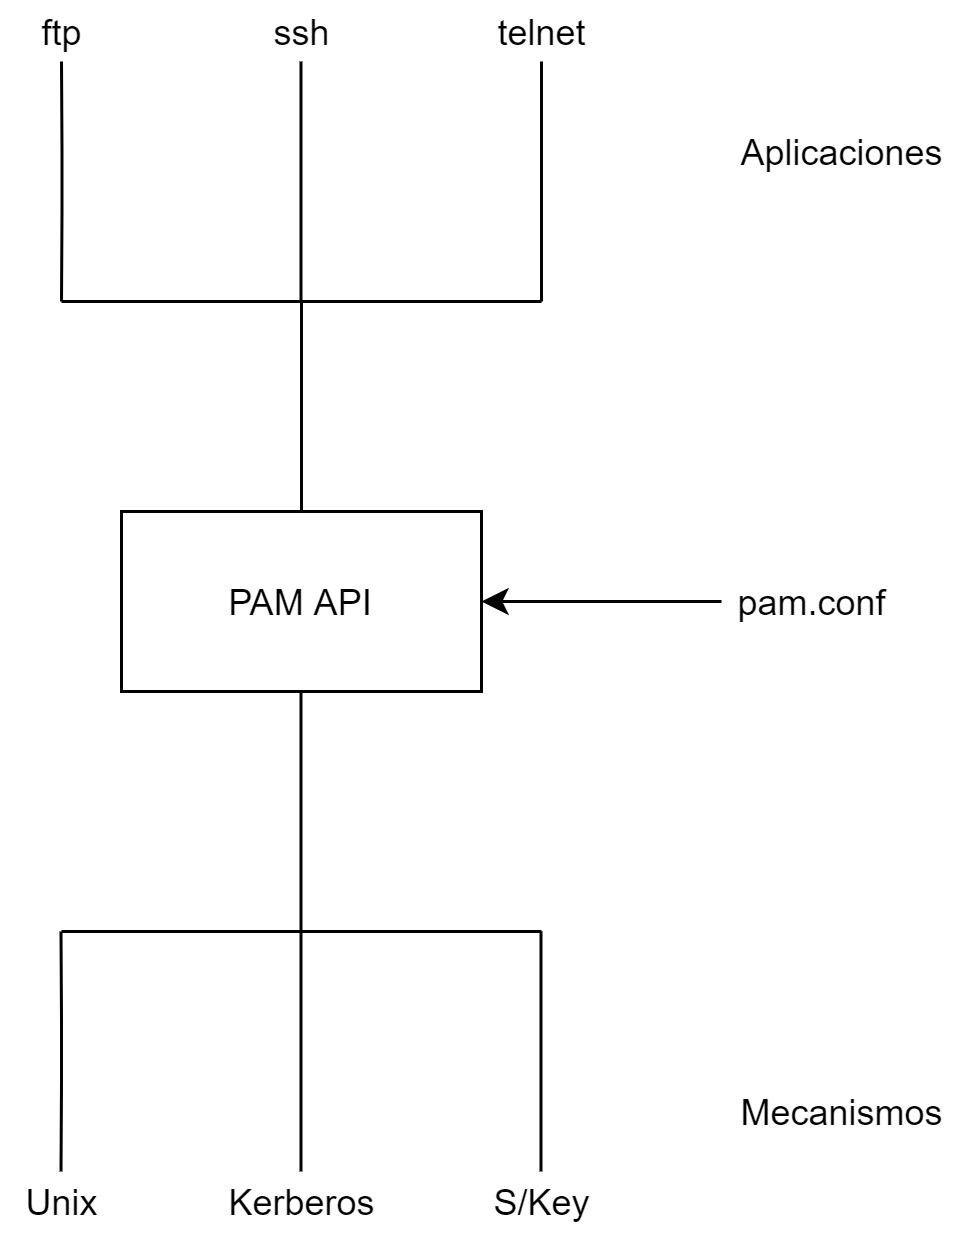
\includegraphics[scale=0.15]{pam_conf.png}
    \caption{Arquitectura básica PAM}
\end{figure}

PAM unifica autenticación y control de acceso al sistema, y permite añadir módulos de autenticación a través de interfaces bien 
definidas. Configuración en la autenticación es un componente junto a administración de cuenta, sesión y contraseñas. Para este 
trabajo, solo se va a usar la parte de autenticación ya que el resto no es necesaria. Cada una de estas áreas funcionales trabajan 
como módulos separados.

Dado la extensión y temática del trabajo, no se pretende dar detalles acerca del funcionamiento de la API de PAM. Simplemente 
anotar que para el desarrollo de este proyecto se usó las siguientes funciones de la API:

\begin{itemize}
    \item \textit{pam\_authenticate()} \cite{pam_sm_authenticate3}: función para autenticar a un usuario
    \item \textit{pam\_get\_user()} \cite{pam_get_user3}: función para obtener el nombre del usuario específico que intenta autenticarse
\end{itemize}

El archivo de configuración PAM (\textit{pam.conf}) es la base de gestión de los módulos. Tal y como se ha mencionado antes, 
cuando una aplicación solicita autenticarse usando algún mecanismo que funcione con PAM, la API comprueba los módulos a ejecutar
en este archivo así como la política que siguen.

El archivo de configuración \ref{code:pam_conf} se ha usado en el broker MQTT de este trabajo. Define los siguientes parámetros 
\cite{mosquittoconf_2021}:

\begin{itemize}
    \item \textit{log\_dest}: ruta absoluta del archivo de logs
    \item \textit{log\_type}: tipo de mensajes a registrar
    \item \textit{log\_timestamp}: añadir valor de marca de tiempo
    \item \textit{include\_dir}: ruta absoluta del directorio de archivos de configuración externos
    \item \textit{listener}: puerto de escucha
    \item \textit{cafile}: ruta absoluta del certificado de la \acf[first-style=short]{ca}
    \item \textit{certfile}: ruta absoluta del certificado del broker MQTT
    \item \textit{keyfile}: ruta absoluta de la clave privada del broker MQTT
    \item \textit{allow\_anonymous}: permitir que clientes se puedan conectar sin proporcionar claves (usuario)
\end{itemize}

El cliente \textit{mosquitto} escucha por defecto por el puerto 1883 para comunicaciones no seguras
y por el 8883 para seguras. El primero solo se usa para comunicaciones internas (\textit{localhost}).

La \acf[first-style=short]{ca} es una entidad que administra certificados digitales, los cuales son usados para vincular una entidad a una 
clave pública. Para el presente tranajo, a diferencia de \cite{multipauthpaper}, se ha usado el broker MQTT como \acf[first-style=short]{ca}. 
No obstante, la \acf[first-style=short]{ca} debe correr en un servidor independiente debido a su papel fundamental en la seguridad de toda
infraestructura y para facilitar la gestión de nodos que se incorporen a la arquitectura del sistema así como revocar aquellos
certificados de clientes que no tengan más acceso.

\section{Análisis de herramientas}
\label{sec:analisis-herramientas}

Para el presente trabajo se ha desarrollado el software usando el lenguaje de programación C dada la facilidad y documentación
disponible a la hora de desarrollar módulos PAM en dicho lenguaje. 
Se ha usado \textit{mosquitto} \cite{eclipse_2018} como cliente MQTT dado su extensa documentación, por ser un software de código 
abierto y estar escrito en C.
Con respecto al entorno de pruebas, se ha usado Vagrant \cite{vagrant} como orquestador de máquinas virtuales para desplegar el 
entorno de prueba.

\chapter{Diseño de la solución}
\label{chap:diseño}

\section{Arquitectura del sistema propuesto}

El sistema propuesto está orientado a ser distribuido y escalable. Además, permite que cualquier aplicación use si esquema de 
autenticación. 
El echo de que use un servidor de autenticación centralizado simplifica la gestión de reglas de acceso y reduce complejidad en 
la revocación de certificados.

En la figura \ref{fig:multauth-diseño} se muestra cómo es la interconexión entre los distintos elementos. A este diseño hay que
añadir dos elementos adicionales: el broker MQTT y el servidor de configuración, tal y como se muestra en \ref{fig:mqtt-topology}.

\begin{figure}[H]
    \centering
    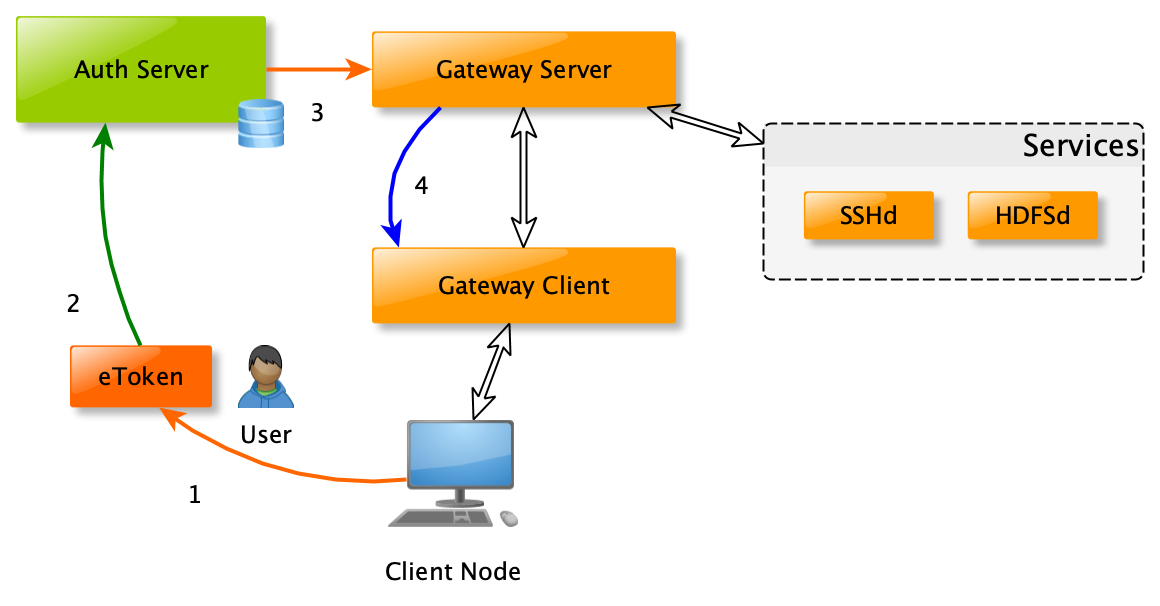
\includegraphics[scale=0.25]{global_topology_v1.png}
    \caption{Diseño del sistema propuesto en \cite{multipauthpaper}}
    \label{fig:multauth-diseño}
\end{figure}

\begin{figure}[H]
    \centering
    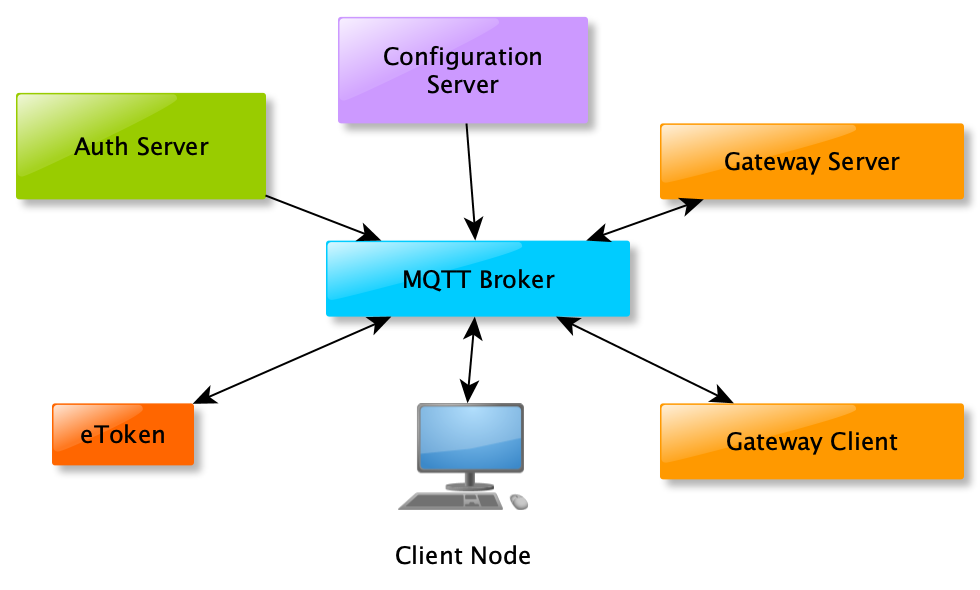
\includegraphics[scale=0.25]{global_topology_mqtt_v1.png}
    \caption{Topología MQTT}
    \label{fig:mqtt-topology}
\end{figure}

\section{Fases de la solución}

La solución propuesta en la sección\ref{sec:motivacion} se ha desarrollado siguiendo las siguientes fases: una primera etapa de preparación de
entorno seguro, una segunda etapa de identificación, y una final de autenticación. Para cada una de las fases se adjunta una 
diagrama de secuencias \footnote{Los valores entre $<$ y $>$ indican un valor en concreto, no el valor definido entre ambos 
símbolos} \footnote{Los tópicos tienen la estructura emisor/receptor/item}

\subsection{Fase TLS}
\label{sec:tls_phase}

En esta fase, el broker MQTT debe crear un certificado firmado por una CA para verificar su identidad. 
Para comunicarse por TLS con el broker MQTT, se ha llevado a cabo los siguientes pasos:

\begin{enumerate}
    \item Crear la clave privada de la CA
    \item Crer el certificado CA usando la clave privada del paso 1 para firmarla
    \item Crear la clave privada del broker MQTT
    \item Crear la solicitud de firma de certificados (\acf[first-style=short]{csr}) para el broker MQTT usando la clave privada del paso 3
    \item Usar la clave y certificado CA para firmar el certificado del broker MQTT
    \item Enviar el certificado del paso 5 al broker MQTT
    \item Distribuir el certificado CA a los cliente que se quieran comunicar a través del broker MQTT 
\end{enumerate}

\begin{figure}[H]
    \centering
    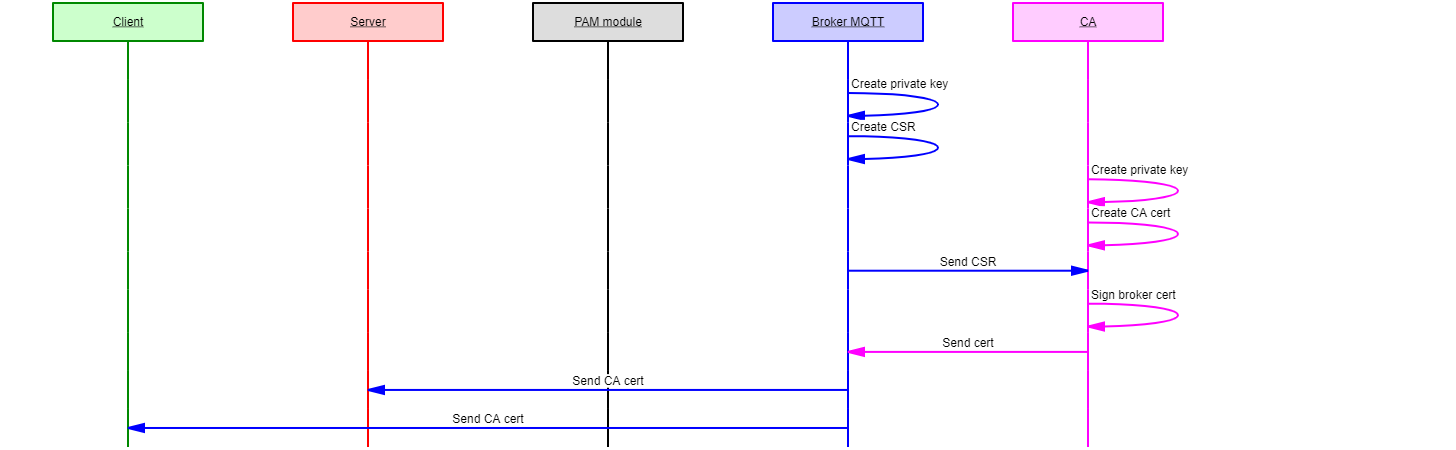
\includegraphics[scale=0.25]{tls_phase.png}
    \caption{Fase TLS}
\end{figure}

Como último paso, el archivo de configuración del cliente \textit{mosquitto} en el broker MQTT tiene que indicar la clave y 
certificados necesarios tal y como figura en \ref{code:pam_conf}.

Si un cliente quiere usar el broker MQTT para publicar un mensaje o subscribrse a un tópico, necesita ``mostrar'' el certificado
CA al broker MQTT. No es la única forma de identificación vía TLS. También existe la opción de que cada cliente
cree su propio certificado firmados por la CA.

\subsection{Fase de identificación}
\label{sec:id_phase}

En esta fase, el cliente se tiene que registrar en el servidor para poder usar su servicio. Para ello, el cliente crea un 
identificador único \acf[first-style=short]{uuid} y un par de claves pública y privada. Estos se guardan en un directorio en concreto. Se ha
escogido \textit{.anubis} en la carpeta \textit{home} del usuario. Las claves se guardan con el UUID como nombre del archivo 
($<uuid>.pem y <uuid>.key$) y finalmente se envía la clave pública al servidor. Se puede usar el protocolo \acf[first-style=short]{scp}. Dado que 
no se quiere usar un método de autenticación distinto al propuesto por este trabajo, se podría crear una clave pública temporal del 
servidor y subirla a algún servidor de claves públicas. El cliente por tanto podría usarla para mandar su clave pública a su 
directorio \textit{.anubis} de forma segura y una vez envíada, eliminarla. Una vez que el servidor tiene la clave pública del 
cliente, este lo registra en el archivo de configuración de usuario \ref{code:user_conf}. Este indica el UUID concreto para un 
usuario en el sistema. Se usa en caso de que el usuario tenga varias claves públicas y por tanto el servidor sepa que clave usar 
para la autenticación.

\begin{figure}[H]
    \centering
    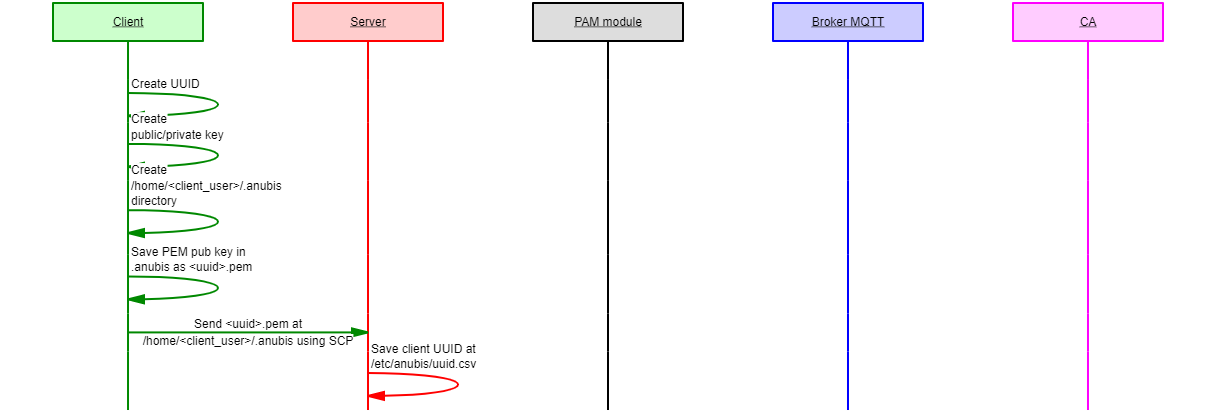
\includegraphics[scale=0.25]{id_phase.png}
    \caption{Fase de identificación}
\end{figure}

\subsection{Fase de autenticación}

En esta fase reside el proces de autenticación del cliente contra el servidor una vez que se ha establecido un canal seguro y 
registrado el cliente en el mismo.

El cliente se subscribe al tópico $pam/<uuid>/challenge$ por el cual recibirá el desafío y envía una petición para 
abrir una sesión por SSH al servidor. 

Al llegar la petición SSH al servidor, este comprueba que almacena el nombre del usuario que se quiere autenticar y comprueba su UUID 
en el archivo de configuración de usuarios \ref{code:user_conf} ($/etc/anubis/uuid.csv$). Este es un archivo de valores separados
por coma (CSV), el usuario y su UUID asignado. Una vez el servidor conoce el UUID, de plantean dos posibilidades:

\begin{enumerate}
    \item Que el usuario no necesite autenticarse de la forma propuesta
    \item Que el usuario tenga que autenticarse
\end{enumerate}

Cada condición se da según la política definida en el archivo de configuración de anubis \ref{code:anubis_conf}. Existen dos 
tipos de políticas:

\begin{enumerate}
    \item \textit{relax}: no es necesario aplicar la autenticación
    \item \textit{strict}: se aplica la autenticación
\end{enumerate}

La política \textit{relax} es útil en casos en los que por ejemplo el usuario provenga de una red de confianza como puede ser una
Universidad. En ese caso, el módulo PAM propuesto devolvería un \textit{PAM\_IGNORE} pasando el siguiente módulo. En caso de la 
política \textit{strict}, es necesario ejecutar el proceso de autenticación propuesto y que devuelva un \textit{PAM\_SUCCESS}.

Una vez que se compruebe el UUID del usuario, si la política es de tipo \textit{strict}, el servidor se subscribe a dos tópicos:

\begin{itemize}
    \item $<uuid>/pam/r$
    \item $<uuid>/pam/s$
\end{itemize}

Por esos tópicos, el cliente publicará el par de valores [$r, s$] del algoritmo ECDSA definido en \ref{subsec:ecdsa} en formato 
hexadecimal.

Seguidamente, crea el desafío y lo publica al tópico $pam/<uuid>/challenge$. El desafio es una cadena de 64 caracteres aleatoria
compuesta de números y letras. Al llegar el mensaje al broker MQTT, este lo reenvía a todos los nodos que estén suscritos a dicho 
tópico. Dado que solo hay un UUID por cliente, el mensaje solo le llega al cliente determinado por el UUID. 

El cliente crea el hash del desafío usando el algoritmo SHA-512 dado su robustez con respecto a otros de menor tamaño como puede 
ser SHA-256. Una vez que tiene el hash, lo firma usando su clave privada creada en \ref{sec:id_phase} y envía ambos valores $[r,s]$ 
por los tópicos $<uuid>/pam/r$ y $uuid>/pam/s$ respectivamente siendo estos retransmitidos por el broker MQTT al servidor.

El servidor recibe ambos valores [$r, s$] para crear la firma de curva elíptica y crea el hash del desafío. A continuación verifica
el hash usando la firma generada anteriormente y la clave pública de tal forma que:

\begin{itemize}
    \item Si el cliente es quien dice ser, la verificación es correcta ya que solo el cliente verídico tiene la clave privada
    \item Si el desafío ha sufrido alguna modificación por la intervención de una tercera persona, la verificación saldrá incorrecta
\end{itemize}

Una verificación correcta devuelve \textit{PAM\_SUCCESS} mientras que una errónea devuelve \textit{PAM\_AUTH\_ERR}, siendo estas 
variables globales de la librería de PAM.  

\begin{figure}[H]
    \centering
    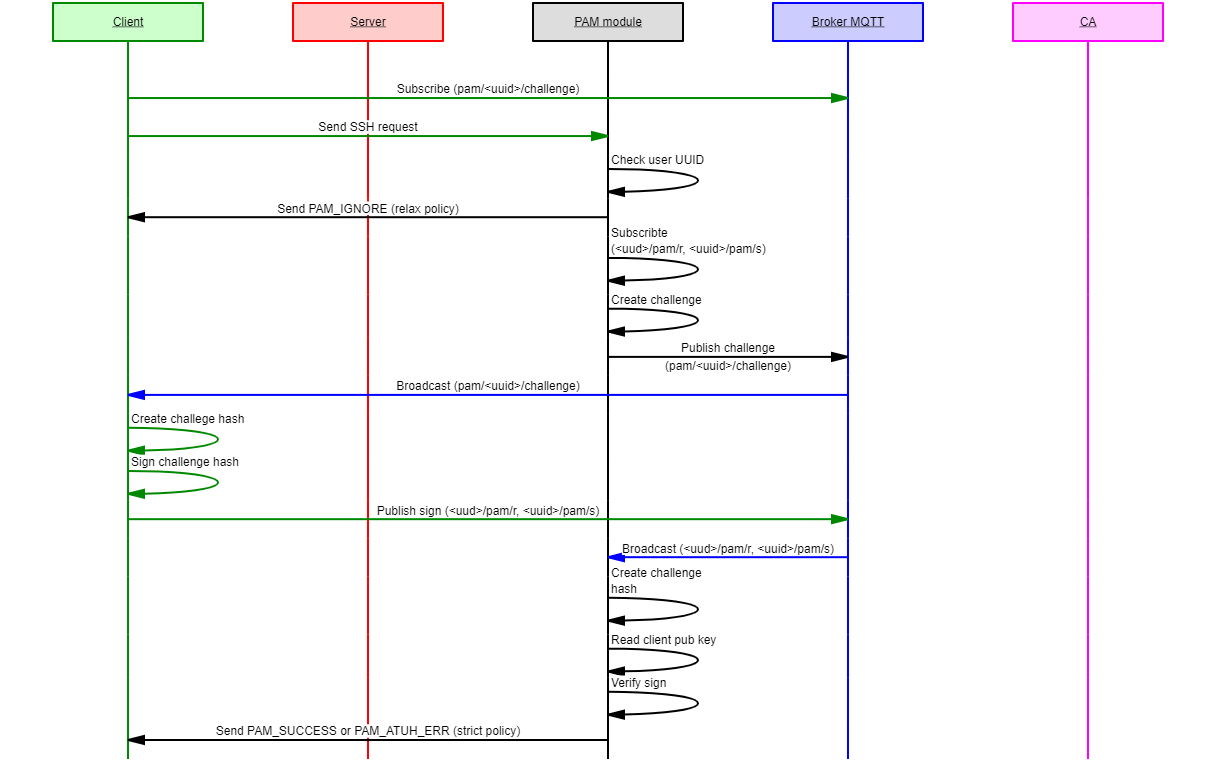
\includegraphics[scale=0.25]{auth_phase.png}
    \caption{Fase de autenticación}
\end{figure}

En la siguiente imagen se mustra la topología global del sistema propuesto:

\begin{figure}[H]
    \centering
    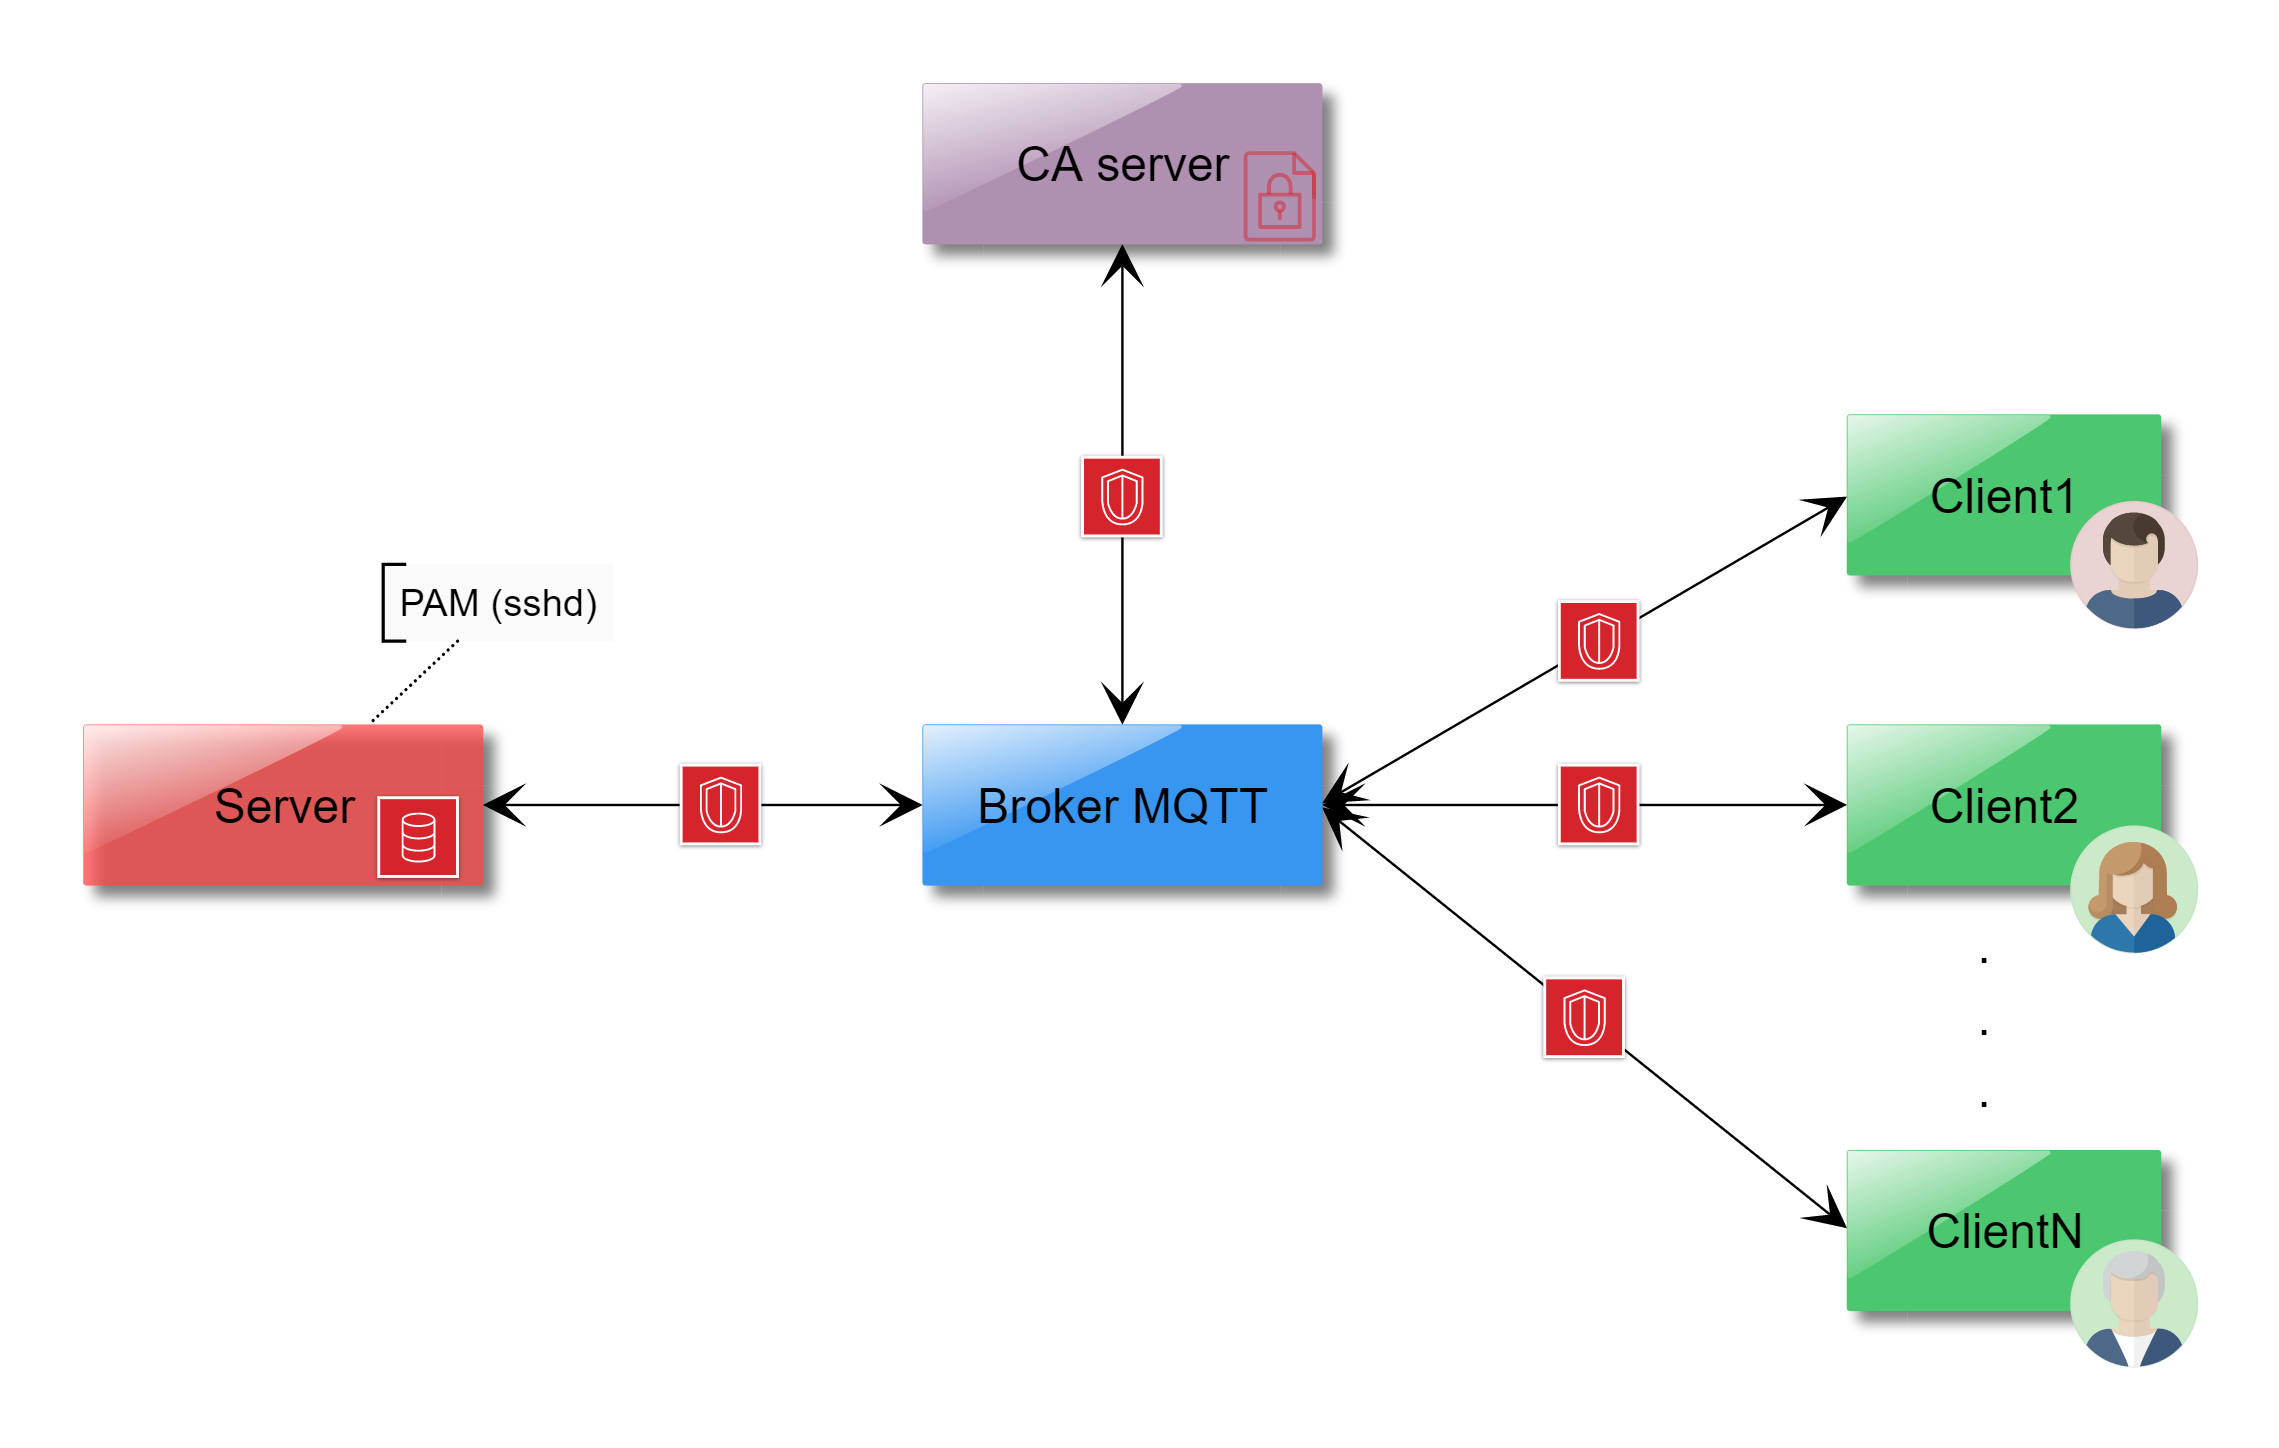
\includegraphics[scale=0.15]{topologia.png}
    \caption{Topología del diseño}
\end{figure}

\section{Código fuente}

El código fuente no se adjunta por simplicidad y limpieza en la memoria pero se encuentra subido a la plataforma de GitHub 
\cite{garcia_sergiogp98mqtt-pam_2021}. 

\section{Entorno de virtualización}

\subsection{Vagrant}

Tal y como se ha mencionado en \ref{sec:analisis-herramientas}, en vez de usar un ESP-32 como eToken de autenticación y un servidor 
físico que recrearía un escenario real, he decido virtualizar el entorno usando máquinas virtuales gracias al programa 
\textit{open-source} de Oracle \textit{Vagrant}.

\textit{Vagrant} es una herramienta destinada a la creación y configuración de entornos de desarrollo. Orginariamente fue 
desarrollado para que trabajase con entornos que corriesen bajo el hipervisor de \textit{VirtualBox} \cite{virtualbox}, siendo 
este un software de virtualización desarrollado por la propia Oracle.

Actualmente $Vagrant$ funciona con otros hpervisores como el de Windows $Hyper-V$, el famoso $VMware$ así como entornos en la 
nube tales como $DigitalOcean$ o $Amazon Web Services$. Está desarrollado en Ruby pero se puede usar en proyectos de diversos 
lenguajes de programación.

Gracias a su facilidad de despliegue y rapidez a la hora de escalar, me ha permitido crear entornos complejos para probar el 
sistema propuesto.

\subsection{Despliegue}

$Vagrant$ require de un archivo de tipo \acf[first-style=short]{yaml} para su configuración que se llama $Vagrantfile$. Para este 
proyecto se ha escrito el siguiente archivo de configuración \ref{code:vagrantfile} compuesto de dos parte:

\begin{enumerate}
    \item El método $add_ssh_key$ añade la clave pública a la máquina virtual creada
    \item La parte de configuración de las máquinas virtuales: broker MQTT, cliente y servidor
\end{enumerate}

Para desplegar una máquina virtual en un Vagrantfile se tiene que especificar una serie de parámetros obligatorios:

\begin{itemize}
    \item Dirección IP privada a usar. Puede ser estática o dinámica (DHCP)
    \item El \textit{Vagrant Box} \cite{vagrant-boxes}. Esta es la imagen del sistema operativo a usar
    \item El proveedor (VirtualBox)
    \item Número y cantidad de memoria CPU
    \item Nombre del hostname 
\end{itemize}

\begin{figure}[H]
    \centering
    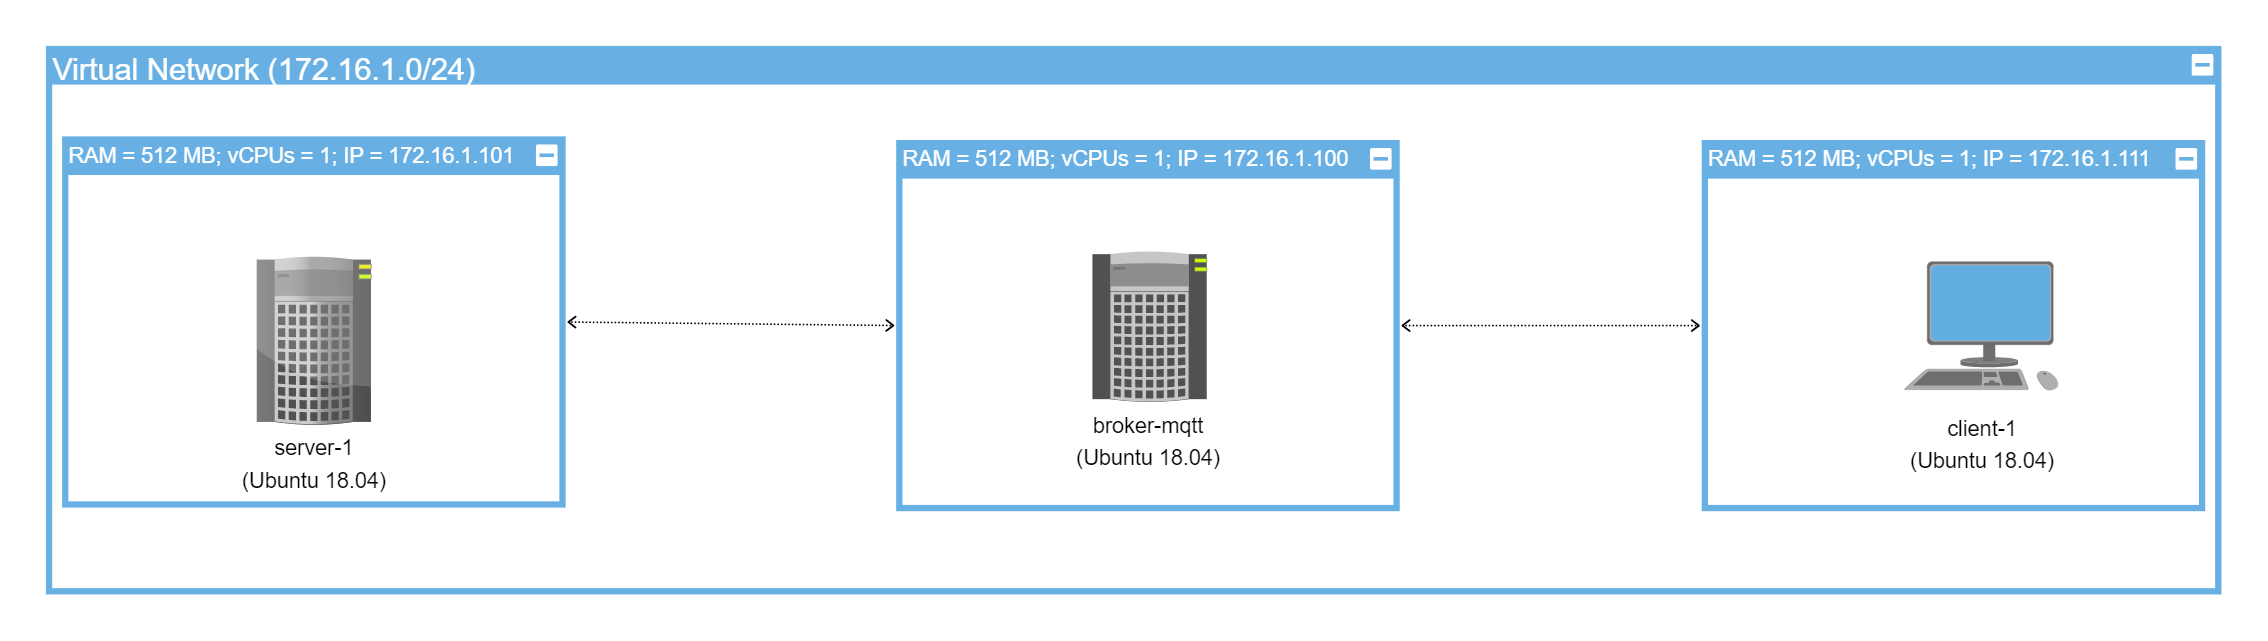
\includegraphics[scale=0.18]{vagrant-topology.png}
    \caption{Topología del entorno virtualizado con Vagrant}
\end{figure}
\cleardoublepage

\chapter{Análisis de seguridad}

Una vez detallado el diseño e implementación del sistema de autenticación propuesto, es necesario conocer la caracterísiticas
de seguridad que implementa. 

\textit{Farooq} propone en \cite{farooq2019elliptic} un sistema similar al propuesto en este trabajo pero centrado en sistemas
electrónicos de tipo contador inteligentes. En él, se hace un estudio de los distintas vulnerabilidades a ciberataques que 
el sistema evita que se sean explotados.

\section{\acrfull{mitm}}

El ataque MITM conocido como ``Ataque de Hombre en el Medio'' es muy común en todo sistema que use una red pública como puede
ser Internet para establecer una comunicación entre dos o más integrantes. 
Para evitar este tipo de ataque, el sistema propuesto usa el algoritmo ECDSA para firmar el desafío y dado que solo el servidor
conoce la clave pública del cliente. En caso de una tercera persona, para que esta se pudiera pasar por el cliente
necesitaría interceptar el desafío y conocer su clave privada para firmarlo. 

\section{Integridad del desafío}

Dado que la respuesta al desafío proviene de la salida de una función hash que ha sido procesada en ambos lados, tanto cliente
como servidor, sin que llege a ser envíada por algún canal, implica que si alguna tercera persona modifica el desafío o la respuesta
a este, el sistema lo detectará y no pasará.

\section{Confidencialidad del mensaje}

Como ya se ha mencionado en \ref{sec:tls_phase}, la comunicación con el broker MQTT se hace vía TLS. Esto permite que los 
mensajes vaya cifrados por una clave. Para usar el broker MQTT y comunicarse con el servidor o viceversa, es necesario presentar
un certificado. Esto garantizar que solo usuario legítimos se comumiquen con el servidor.





\cleardoublepage

\chapter{Presupuesto}

\section{Componentes hardware y software}

Para la realización de este proyecto no se ha usado dispositvos hardware dedicados como podría ser un Arduino o Raspberry.
Simplemente se ha virtualizado el entorno de pruebas mediante software de vitualización (VirtualBox) y por tanto no ha tenido
coste económico ninguno. En cuanto al software, tampoco se han usado programas con licencias ya que tanto el cliente MQTT 
(mosquitto), la API de SSL y el entorno de desarrollo (Visual Studio Code) son de código libre.

\section{Diagrama de Gantt}

\begin{figure}[H]
    \centering
    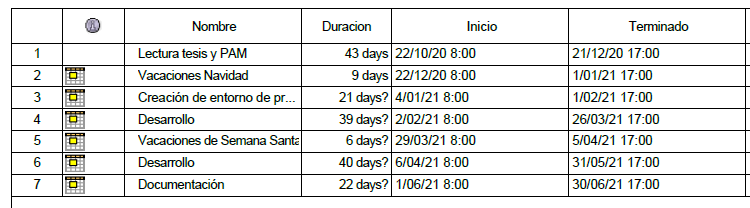
\includegraphics{diagrama-gantt.png}
    \caption{Diagrama de Gantt}
\end{figure}

\cleardoublepage

\chapter{Conclusión}

\section{Trabajo futuro}


\cleardoublepage

\addappheadtotoc

\appendix

\chapter{Archivos de configuración}

\begin{lstlisting}[style=Consola, caption={Archivo de configuración PAM}, label={code:pam_conf}]
    # Place your local configuration in /etc/mosquitto/conf.d/
    #
    # A full description of the configuration file is at
    # /usr/share/doc/mosquitto/examples/mosquitto.conf.example
    pid_file /run/mosquitto/mosquitto.pid

    log_dest file /var/log/mosquitto/mosquitto.log
    log_type all
    log_timestamp true

    include_dir /etc/mosquitto/conf.d

    listener 1883 localhost
    listener 8883

    cafile /etc/mosquitto/ca_certificates/ca.crt
    certfile /etc/mosquitto/certs/broker-mqtt.crt
    keyfile /etc/mosquitto/certs/broker-mqtt.key

    allow_anonymous true
\end{lstlisting}

\begin{lstlisting}[style=Consola, caption={Archivo de configuración de usuarios en /etc/anubis/uuid.csv}, label={code:user_conf}]
    username,uuid
    client-1,68263723-e928-4f71-8339-c609478f0a1a   
\end{lstlisting}

\begin{lstlisting}[style=Consola, caption={Archivo de configuración anubis en /etc/anubis/anubis.conf}, label={code:anubis_conf}]
    # ------------------------#
    # /etc/anubis/anubis.conf
    # ------------------------#
    #
    # NOTE
    # ----
    #
    # Configuration file for MQTT-PAM module used to authenticate via SSH
    # Use only a space between key and value
    #
    # Permitted values:
    # access_type [relax, strict]
    # ip_address 150.214.*.*
    # ------------------------#
    #
    # Format:
    # key value

    access_type relax   
\end{lstlisting}

\begin{lstlisting}[style=Consola, caption={Petición SSH cliente al servidor}, label={code:ssh-request}]
    vagrant@client-1:~$ ssh client-1@172.16.1.101
    client-1@172.16.1.101's password:
    Found UUID in user client-1: 68263723-e928-4f71-8339-c609478f0a1a
    Client server_2941 sending CONNECT
    Client server_2941 sending SUBSCRIBE (Mid: 1, Topic: 68263723-e928-4f71-8339-c609478f0a1a/pam/r, QoS: 0, Options: 0x00)
    Client server_2941 sending SUBSCRIBE (Mid: 1, Topic: 68263723-e928-4f71-8339-c609478f0a1a/pam/s, QoS: 0, Options: 0x00)
    Client server_2941 sending PUBLISH (d0, q0, r0, m2, 'pam/68263723-e928-4f71-8339-c609478f0a1a/challenge', ... (64 bytes))
    Client server_2941 received CONNACK (0)
    Client server_2941 received SUBACK
    Client server_2941 received PUBLISH (d0, q0, r0, m0, '68263723-e928-4f71-8339-c609478f0a1a/pam/r', ... (130 bytes))
    Client server_2941 received PUBLISH (d0, q0, r0, m0, '68263723-e928-4f71-8339-c609478f0a1a/pam/s', ... (130 bytes))
    Successfully verified
    Exiting...
    Client server_2941 sending DISCONNECT
    PAM OK
    Welcome to Ubuntu 20.04.2 LTS (GNU/Linux 5.4.0-74-generic x86_64)

    * Documentation:  https://help.ubuntu.com
    * Management:     https://landscape.canonical.com
    * Support:        https://ubuntu.com/advantage

    System information as of Mon Jun 21 21:19:03 UTC 2021

    System load:  0.0               Processes:               109
    Usage of /:   7.0% of 38.71GB   Users logged in:         1
    Memory usage: 41%               IPv4 address for enp0s3: 10.0.2.15
    Swap usage:   0%                IPv4 address for enp0s8: 172.16.1.101

    * Super-optimized for small spaces - read how we shrank the memory
    footprint of MicroK8s to make it the smallest full K8s around.

    https://ubuntu.com/blog/microk8s-memory-optimisation

    38 updates can be applied immediately.
    To see these additional updates run: apt list --upgradable


    Last login: Mon Jun 21 21:11:24 2021 from 172.16.1.111
    client-1@server-1:~$
\end{lstlisting}

\begin{lstlisting}[style=Consola, caption={Salida script cliente}, label={code:client-script}]
    vagrant@client-1:~/tfg/bin$ ./client broker.mqtt.com 8883 68263723-e928-4f71-8339-c609478f0a1a /etc/mosquitto/ca_certificates/ca.crt
    Client 68263723-e928-4f71-8339-c609478f0a1a sending CONNECT
    Client 68263723-e928-4f71-8339-c609478f0a1a sending SUBSCRIBE (Mid: 1, Topic: pam/68263723-e928-4f71-8339-c609478f0a1a/challenge, QoS: 0, Options: 0x00)
    Listening to pam/68263723-e928-4f71-8339-c609478f0a1a/challenge topic...
    Client 68263723-e928-4f71-8339-c609478f0a1a received CONNACK (0)
    Client 68263723-e928-4f71-8339-c609478f0a1a received SUBACK
    Client 68263723-e928-4f71-8339-c609478f0a1a received PUBLISH (d0, q0, r0, m0, 'pam/68263723-e928-4f71-8339-c609478f0a1a/challenge', ... (64 bytes))
    Received challenge: ITOeM0joCRNR5dm.hWS5O7BaxvE8UdE7SMoPKoQck5WhhYu1di2KrBrxGsG6o76
    Client 68263723-e928-4f71-8339-c609478f0a1a sending PUBLISH (d0, q0, r0, m2, '68263723-e928-4f71-8339-c609478f0a1a/pam/r', ... (130 bytes))
    Client 68263723-e928-4f71-8339-c609478f0a1a sending PUBLISH (d0, q0, r0, m3, '68263723-e928-4f71-8339-c609478f0a1a/pam/s', ... (130 bytes))
    Exiting...
    Client 68263723-e928-4f71-8339-c609478f0a1a sending DISCONNECT
\end{lstlisting}

\begin{lstlisting}[style=Consola, caption={Archivo de configuración PAM para sshd}, label={code:pam-sshd}]
    # PAM configuration for the Secure Shell service

    # MQTT PAM module
    auth required mqtt-pam.so broker.mqtt.com 8883 /etc/mosquitto/ca_certificates/ca.crt

    # Standard Un*x authentication.
    @include common-auth

    # Disallow non-root logins when /etc/nologin exists.
    account    required     pam_nologin.so

    # Uncomment and edit /etc/security/access.conf if you need to set complex
    # access limits that are hard to express in sshd_config.
    # account  required     pam_access.so

    # Standard Un*x authorization.
    @include common-account

    # SELinux needs to be the first session rule.  This ensures that any
    # lingering context has been cleared.  Without this it is possible that a
    # module could execute code in the wrong domain.
    session [success=ok ignore=ignore module_unknown=ignore default=bad]        pam_selinux.so close

    # Set the loginuid process attribute.
    session    required     pam_loginuid.so

    # Create a new session keyring.
    session    optional     pam_keyinit.so force revoke

    # Standard Un*x session setup and teardown.
    @include common-session

    # Print the message of the day upon successful login.
    # This includes a dynamically generated part from /run/motd.dynamic
    # and a static (admin-editable) part from /etc/motd.
    session    optional     pam_motd.so  motd=/run/motd.dynamic
    session    optional     pam_motd.so noupdate

    # Print the status of the user's mailbox upon successful login.
    session    optional     pam_mail.so standard noenv # [1]

    # Set up user limits from /etc/security/limits.conf.
    session    required     pam_limits.so

    # Read environment variables from /etc/environment and
    # /etc/security/pam_env.conf.
    session    required     pam_env.so # [1]
    # In Debian 4.0 (etch), locale-related environment variables were moved to
    # /etc/default/locale, so read that as well.
    session    required     pam_env.so user_readenv=1 envfile=/etc/default/locale

    # SELinux needs to intervene at login time to ensure that the process starts
    # in the proper default security context.  Only sessions which are intended
    # to run in the user's context should be run after this.
    session [success=ok ignore=ignore module_unknown=ignore default=bad]        pam_selinux.so open

    # Standard Un*x password updating.
    @include common-password
\end{lstlisting}

\begin{lstlisting}[language=Ruby, caption={Archivo de configuración Vagrantfile}, label={code:vagrantfile}]
    n_servers = 2
    n_clients = 1
    
    server_net = "172.16.1.10"
    client_net = "172.16.1.11"
    broker_mqtt_net = "172.16.1.100"
    
    def add_ssh_key(config)
        ssh_pub_key = File.readlines("#{Dir.home}/.ssh/id_rsa.pub").first.strip
        config.vm.provision "shell" do |s|
          s.inline = <<-SHELL
            echo #{ssh_pub_key} >> /home/vagrant/.ssh/authorized_keys
            mkdir -p /root/.ssh/
            chmod 700 /root/.ssh/
            echo #{ssh_pub_key} >> /root/.ssh/authorized_keys
          SHELL
        end
    end
    
    Vagrant.configure("2") do |config|
        config.vm.synced_folder ".", "/home/vagrant/tfg"
    
        (1..n_servers).each do |i|
            config.vm.define "server-#{i}" do |node|
                node.vm.network :private_network, ip: "#{server_net}#{i}"
                node.vm.box = "ubuntu/focal64"
                node.vm.provider "virtualbox" do     |pmv|
                    pmv.memory = 512
                    pmv.cpus   = 1
                end
                node.vm.hostname = "server-#{i}"
                add_ssh_key(config)
            end
        end
    
        (1..n_clients).each do |i|
            config.vm.define "client-#{i}" do |node|
                node.vm.network :private_network, ip: "#{client_net}#{i}"
                node.vm.box = "ubuntu/focal64"
                node.vm.provider "virtualbox" do |pmv|
                    pmv.memory = 512
                    pmv.cpus   = 1
                end
                node.vm.hostname = "client-#{i}"
                add_ssh_key(config)
            end
            
        end
    
        config.vm.define "broker-mqtt" do |node|
            node.vm.network :private_network, ip: "#{broker_mqtt_net}"
            node.vm.box = "ubuntu/focal64"
            node.vm.provider "virtualbox" do |pmv|
                pmv.memory = 512
                pmv.cpus   = 1
            end
            node.vm.hostname = "broker-mqtt"
            add_ssh_key(config)
        end
    end        
\end{lstlisting}


\cleardoublepage

\bibliographystyle{unsrt}
\bibliography{bibliografia.bib}

\clearpage

\addcontentsline{toc}{chapter}{Acrónimos}
\printacronyms[name=Acrónimos]

\end{document}